\documentclass[border=8pt]{standalone}
\usepackage{mathpazo}
\usepackage{pgfplots}
\pgfplotsset{compat=1.18}

\definecolor{stblue}{HTML}{7B97AD}
\definecolor{rwgold}{HTML}{B8995E}
\definecolor{sage}{HTML}{7A9A7E}
\definecolor{terracotta}{HTML}{C47A6A}
\definecolor{dkbrown}{HTML}{3D3530}
\definecolor{wmgray}{HTML}{7B7067}
\definecolor{lavender}{HTML}{907EA0}

\begin{document}
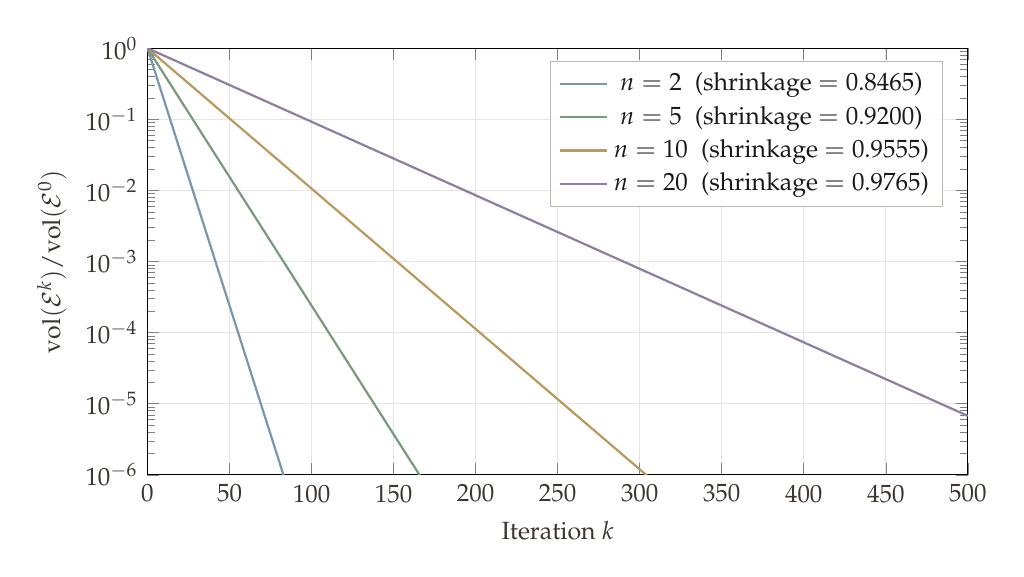
\begin{tikzpicture}
\begin{semilogyaxis}[
  width=12cm, height=7cm,
  xlabel={Iteration $k$},
  ylabel={$\mathrm{vol}(\mathcal{E}^k) / \mathrm{vol}(\mathcal{E}^0)$},
  xmin=0, xmax=500,
  ymin=1e-6, ymax=1,
  grid=major,
  grid style={gray!20},
  legend pos=north east,
  legend style={font=\small, fill=white, fill opacity=0.9, draw=wmgray!50},
  tick label style={font=\small, color=dkbrown},
  label style={font=\small, color=dkbrown},
  every axis plot/.append style={thick},
]

% n=2: shrinkage = exp(-1/(2*3)) = exp(-1/6) ≈ 0.8465
\addplot[stblue, domain=0:500, samples=100]
  {exp(-x/(2*(2+1)))};
\addlegendentry{$n=2$\; (shrinkage $= 0.8465$)}

% n=5: shrinkage = exp(-1/(2*6)) = exp(-1/12) ≈ 0.9200
\addplot[sage, domain=0:500, samples=100]
  {exp(-x/(2*(5+1)))};
\addlegendentry{$n=5$\; (shrinkage $= 0.9200$)}

% n=10: shrinkage = exp(-1/(2*11)) = exp(-1/22) ≈ 0.9555
\addplot[rwgold, domain=0:500, samples=100]
  {exp(-x/(2*(10+1)))};
\addlegendentry{$n=10$\; (shrinkage $= 0.9555$)}

% n=20: shrinkage = exp(-1/(2*21)) = exp(-1/42) ≈ 0.9765
\addplot[lavender, domain=0:500, samples=100]
  {exp(-x/(2*(20+1)))};
\addlegendentry{$n=20$\; (shrinkage $= 0.9765$)}

\end{semilogyaxis}
\end{tikzpicture}
\end{document}
